\documentclass[11pt, oneside]{article} 
\usepackage{geometry}
\geometry{letterpaper} 
\usepackage{graphicx}
	
\usepackage{amssymb}
\usepackage{amsmath}
\usepackage{parskip}
\usepackage{color}
\usepackage{hyperref}

\graphicspath{{/Users/telliott/Dropbox/Github-Math/geoproof/figures/}{/Users/telliott/Dropbox/Github-Math/figures/}}
% \begin{center} \includegraphics [scale=0.4] {gauss3.png} \end{center}


\title{Similar triangles}
\date{}

\begin{document}
\maketitle
\Large

%[my-super-duper-separator]

\subsection*{equal angles $\rightarrow$ parallel}

When two triangles are \emph{similar}, they have the same shape but are scaled differently.  By the same shape, we mean they have the same three angles.  

Because the angles are the same, we can draw the two triangles nestled inside one another, picking any of the three angles as the common vertex.

In the figure, $\triangle ABC \sim \triangle ADE$ ($\sim$ is the symbol for similarity).
\begin{center} 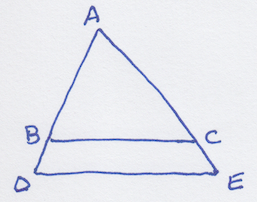
\includegraphics [scale=0.5] {A1.png} \end{center}

And because the angles are the same, say, $\angle ABC = \angle D$, it follows that $BC \parallel DE$ by the converse of alternate interior angles.

\subsection*{similar sides in a right triangle}

There are other properties that go along with similarity.  We will prove that for similar right triangles, all angles equal implies equal ratios of sides.  Our approach is from Acheson and is based on an observation about area.

Draw a rectangle and one diagonal and pick a point on the diagonal
\begin{center} 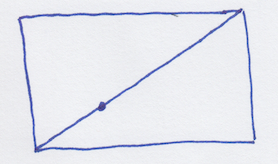
\includegraphics [scale=0.5] {A5.png}
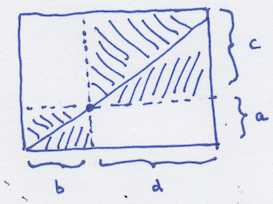
\includegraphics [scale=0.5] {A6.png} \end{center}

All of the right triangles in the figure are similar.  The ones have a shared length of the diagonal are congruent. This part is easily proved with the alternate interior angles theorem, then use complementary angles in a right triangle, and finish with vertical angles.  

By changing the height of the figure, we can obtain any two complementary angles we wish.  And by changing the placement of the central point we can get any ratio.

Finally, the two shaded rectangles are bisected by the diagonal. This is a basic property of rectangles;  we have congruent $\triangle$ by SSS).  So both pairs of congruent triangles have equal area.

But the big triangles formed by the diagonal are also congruent and also have equal area.

Therefore, we just subtract equal areas to find that the two unshaded rectangles above and below the diagonal are equal in area.  The one on top has area $bc$ and the one below has area $ad$.  We have

\[ bc = ad \]
\[ \frac{a}{c} = \frac{b}{d} \]

A bit of algebra gives:
\[ \frac{a}{c} + \frac{c}{c} = \frac{b}{d} + \frac{d}{d} \]
\[ \frac{a + c}{c} = \frac{b + d}{d} \]
\[ \frac{a + c}{b + d} = \frac{c}{d} = \frac{a}{b} \]

We have added one to each side before the rearrangement, maintaining equality.

\subsection*{hypotenuse}

It is natural to ask, what about the hypotenuse?  There is an algebraic proof based on the Pythagorean theorem.  However, our easiest proof of the Pythagorean theorem is based on similarity.  It would be a circular (and logically invalid) argument!

Luckily, we have Euclid's proof of the Pythagorean theorem, which uses SAS, and this would get us out of the trap.  So, we could prove that similar right triangles have equal ratios of hypotenuse as well as sides, and then extend that proof to all triangles by dissecting them into right triangles.  

But we have two terrific proofs from Euclid so why not just go ahead to the general case.

$\square$\subsection*{all similar triangles}

\begin{center} 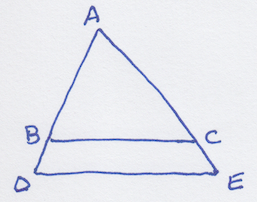
\includegraphics [scale=0.5] {A1.png} \end{center}
Above, $BC \parallel DE$ ($BC$ is parallel to $DE$).  In addition, we have equal ratios of sides.
\[ \frac{AB}{AD} = \frac{BC}{DE} = \frac{AC}{AE} \]
and
\[ \frac{AB}{BD} = \frac{BC}{DE - BC} = \frac{AC}{CE} \]
The second set of ratios is easily derived from the first exactly as we did before.
\begin{center} 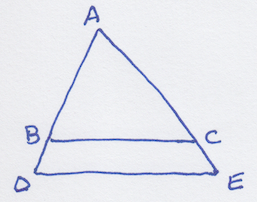
\includegraphics [scale=0.5] {A1.png} \end{center}

\subsection*{parallel $\rightarrow$ equal ratios}

Given:  $BC \parallel DE$.  We claim that the ratios given above follow.

Notice that $C$ is a vertex of both $\triangle ABC$ and $\triangle BCD$.  Therefore, the altitude from C to $ABD$ is the same for both triangles.

\begin{center} 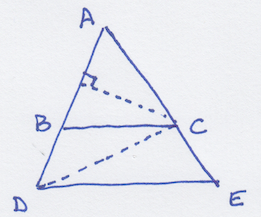
\includegraphics [scale=0.6] {A3.png} \end{center}
If we define the symbol $(ABC)$ to mean area, then
\[ \frac{(ABC)}{(BCD)} = \frac{AB}{BD} \]
The areas of the two triangles are in the same ratio as the lengths of the bases, since the altitudes are the same.

A symmetric construction 
\begin{center} 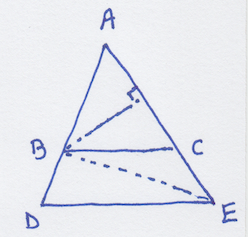
\includegraphics [scale=0.6] {A4.png} \end{center}
shows that
\[ \frac{(ABC)}{(BCE)} = \frac{AC}{CE} \]

However, $(BCD) = (BCE)$.  The two triangles have the same base, $BC$, and their altitudes are the same because the respective vertices at $D$ and $E$ lie on the same line parallel to $BC$.

Therefore the first two expressions from above are equal.
 \[ \frac{(ABC)}{(BCD)} = \frac{AB}{BD} \]
 \[ \frac{(ABC)}{(BCE)} = \frac{AC}{CE} \]

 Since $(BCD) = (BCE)$, the left-and sides are identical, therefore, so are the right-hand sides.
 \[ \frac{AB}{BD} = \frac{AC}{CE} \]

 $\square$
  
 \subsection*{equal ratios $\rightarrow$ parallel}
 
Given that $\triangle ABC$ has equal ratios to $\triangle ADE$.
\[ \frac{AB}{BD} = \frac{AC}{CE} = \frac{BC}{DE} \]

We claim that $BC \parallel DE$.  
\begin{center} 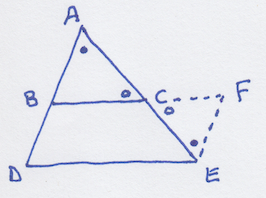
\includegraphics [scale=0.6] {A2.png} \end{center}

Just to be clear, we are allowed to use the previous theorem to help us prove its converse.  Given all 3 angles equal, it follows that equal ratios of the sides obtains.  We will then use equal ratios to prove the parallel property.

\emph{Proof}.

First, draw $EF$ extending up from $E$, with $EF \parallel ABD$.  

Alternate interior angles gives us that $\angle A$ is equal to $\angle CEF$, marked with filled dots.  Another angle equality is at vertex $C$, by vertical angles.  Since two angles are equal, all three are, and this means that all three sides are in equal ratios by the previous theorem.

Since $\triangle ABC \sim \triangle CEF$
\[ \frac{AB}{EF} = \frac{AC}{CE} = \frac{BC}{CF} \]
but we were given that
\[ \frac{AC}{CE} = \frac{AB}{BD} \]
so
\[ BD = EF \]
\begin{center} 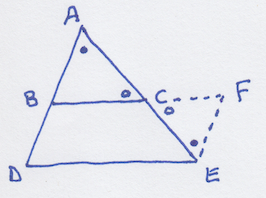
\includegraphics [scale=0.6] {A2.png} \end{center}

We have $BD = EF$ and we started with $BD \parallel EF$.  This is enough to establish that BCED is a parallelogram.  Therefore $BCF \parallel DE$.

We also have
\[ \frac{BC}{BF} = \frac{AC}{AE} = \frac{BC}{DE} \]

So $BF = DE$, as expected for a parallelogram.

$\square$

\subsection*{median theorem}

Draw a line segment from the right angle of a right $\triangle$ to the hypotenuse, such that it is the median,  that is $AD = DC$.  Prove that $BD$ is also equal to $AD$ and $DC$.
\begin{center} 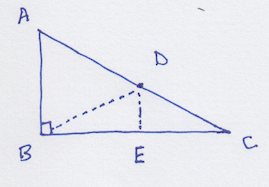
\includegraphics [scale=0.7] {D9.png} \end{center}

\emph{Proof}.

Here's a standard approach using similar triangles.  Drop the perpendicular from $D$ to $E$.  By similar triangles, since $AD = DC$, $BE = EC$.  So $\triangle BDE \cong \triangle DCE$.

It follows that $BD = DC$, $\triangle BDC$ is isosceles, and so is $\triangle ABD$.

$\square$

Even better, use the converse of Thales' theorem.  

\emph{Proof}.

Since $\angle ABC$ is a right angle, we can draw it in a triangle with $AC$ as the diameter.  We are given that $AD = DC$.

Since $B$ is on the circle and $D$ is the center of the circle, $BD$ is also a radius.

$\square$

Still better, a proof without words.
\begin{center} 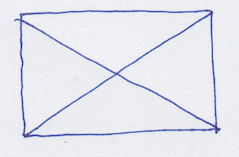
\includegraphics [scale=0.7] {D10.png} \end{center}

With words:  draw a second right $\triangle$ to form a rectangle.  The diameters of any rectangle cross at the midpoints of each.

\emph{Proof}.

The triangles on top and bottom are congruent (SSS).  Therefore the two diameters are bisected.

$\square$

\subsection*{Pythagorean theorem}

Similarity allows a very simple proof of the theorem.

\emph{Proof}.

Place two identical right triangles next to each other so that the sides $b$ and $a$ lie along one straight line.
\begin{center} \includegraphics [scale=0.35] {pyth16.png} \end{center}
Now, scale the triangles so that the sides have identical length.  An easy way to do that is to multiply each side length on the left by $b$, and each one on the right by $a$.
\begin{center} \includegraphics [scale=0.4] {pyth18.png} \end{center}

$\circ$ \ The entire figure forms a rectangle (two opposing sides equal, two adjacent right angles), and also forms a third triangle.

$\circ$ \ $\theta$ is a right angle, since its neighbors are complementary and altogether they add to two right angles.  The bottom two angles of the rectangle are complementary to their neighbors.  So the third triangle has the same angles as the first two.  It is similar.

$\circ$ \ The scale factor for the third triangle is $c$, so the length of the opposite side of the rectangle is $cc$

Since the two long sides of a rectangle are also equal in length:
\[ a^2 + b^2 = c^2 \]

$\square$

\subsection*{pyramid height}

Thales was from Miletus and he lived around 600 BC.  He is believed to have traveled extensively and was likely of Phoenician heritage.  As you probably know, the Phoenicians were famous sailors who founded many settlements around the Mediterranean.  

They competed with the mainland Greeks and later with the Romans for colonies, and their major city, Carthage, was destroyed much later by the Romans, in the third Punic War.  Hannibal rode his famous elephants over the Alps in the second Punic war.

During his travels, Thales went to Egypt, home to the great pyramids at Giza, which were already ancient then.  They had been built about 2560 BC (dated by reference to Egyptian kings) and were already 2000 years old at that time!

The story is that Thales asked the Egyptian priests about the height of the Great Pyramid of Cheops, and they would not tell him.  So he set about measuring it himself.  He used similar triangles.  I'm sure he wrote down his answer, but I'm not aware that it survives.  The current height is 480 feet.

\begin{center} \includegraphics [scale=0.25] {Thales_theorem_6.png} \end{center}

Plutarch says this:

\begin{quote}the king finds much to admire in you, and in particular he was immensely pleased with your method of measuring the pyramid, because, without making any ado or asking for any instrument, you simply set your walking stick upright at the edge of the shadow which the pyramid cast, and, two triangles being formed by the intercepting of the sun's rays, you demonstrated that the height of the pyramid bore the same relation to the length of the stick as the one shadow to the other.\end{quote}

So the actual method is even cleverer than the diagram shows.


\end{document}
